
%%%%%%%%%%%%%%%%%%%%%%%%%%%%%%%%%%%%%%%%%%%%%%%%%%%%%%%%%%%%%%%%%%%%%%%
%                           Fourth Chapter                            %
%                       New Posture Generation                        %
%%%%%%%%%%%%%%%%%%%%%%%%%%%%%%%%%%%%%%%%%%%%%%%%%%%%%%%%%%%%%%%%%%%%%%%

\chapter{New Posture Generation}

%\section{List of contributions}
%\begin{itemize}
  %\item{Posture Generation, variables and architecture}
    %\begin{itemize}
      %\item Geometric expressions:
        %\begin{itemize}
          %\item Represent everything based on frames
          %\item Automatic derivative computation
        %\end{itemize}
      %\item Automatic mapping
      %\item Problem generator: a posture generation problem factory
    %\end{itemize}
  %\item{Problem Formulation: formulation of usual problems in the geometric expressions framework}
    %\begin{itemize}
      %\item Contact with plane surface
      %\item Static equilibrium: Newton/CoM projection
      %\item Forces in friction cones
      %\item Articular limits
      %\item Torque limits
      %\item Torque minimization
      %\item Goal Posture
    %\end{itemize}
  %\item{Implementation of new types of constraints in our formulation}
    %\begin{itemize}
      %\item Contact with parametrized surfaces on Rn
      %\item Contact with parametrized surfaces on S2: Sphere, SuperEllipsoid
      %\item Contact with Catmull-Clark Subdivision surfaces
    %\end{itemize}
  %\item{Contact with desired force}
  %\item{Potential contacts}
  %\item{Simulation Results}
  %\item{Multi-Robot}
%\end{itemize}

Writing a posture generation problem can easily become cumbersome without the appropriate tools.
Common pitfalls are for example writing the derivative of a function, managing how the Jacobian matrices of the already implemented functions are modified when a variable is added to the problem, adding a new type of constraint, or correctly writing a function on a sub-manifold of the problem manifold.
A fair amount of bookkeeping is always necessary, which should not be the charge of the user writing the constraints.
In our PG, we propose an architecture automating most of the problematic tasks, so that the user can focus on the mathematical formulation of the problem:
\begin{itemize}
  \item A system of geometrical and mathematical expression trees that automatically computes the mathematical expressions behind geometric relations
  \item An automatic mapping between the submanifold of each function and the global manifold of the problem
  \item A problem generator that aggregates all the informations from the abovementionned items to generate an optimization problem that can be passed to the solver
\end{itemize}


\section{Geometric expressions}
\label{sec:geometric_expressions}

Most constraints are geometric.
In order to simplify the writing of functions, we use a dedicated system of expression graph encapsulated in a set of geometric objects.
The main idea is to separate the purely mathematical logic from the geometric one.
As an example if $P_r$ and $V_r$ are a point and a vector attached to the camera of the robot, and $P_e$ is a fixed point in the environment, the constraint $(P_e - P_r).V_r = 0$ can be used to have the robot look at $P_e$.
With our system, the user creates only those objects and write the code {\tt (Pe-Pr).dot(Vr)} to get the value needed.
The geometric layer takes care that all the quantities are expressed in the correct frame, the mathematical layer performs the corresponding operations.
If $q$ is a variable object, {\tt (Pe-Pr).dot(Vr).diff(q)} returns automatically the differential of the expression w.r.t. $q$. This makes the writing of the constraints very easy.

At the mathematical level, we consider 5 types of expressions which can be either variables or constants:
\begin{itemize}
  \item Scalar, a 1-dimensional element of $\mathbb{R}$
  \item Coordinates, a 3-dimensional element of $\mathbb{R}^3$
  \item Rotation, a $3\times3$ matrix representing a 3D rotation
  \item Transformation, a $4\times4$ matrix representation of a 3D isometry
  \item Array, a dynamic size array
\end{itemize}
The meaningful unary (inverse, opposite, norm\ldots) and binary (multiplication, addition, subtraction, dot product\ldots) operations (with their derivatives by chain rule) are implemented.
We also have a Function class for more complicated expressions, for example expressing $q \mapsto T_i(q)$ where $T_i$ is the transformation between the reference frame of the robot and the frame of its $i$-th body~\footnote{The kinematics of rigid body systems is handled by the RBDyn library (\url{https://github.com/jorisv/RBDyn})}.
The combinations of those elementary operations defines a computation graph, just like in many symbolic calculation frameworks.

The geometric layer consists of physical or geometric objects, named features, which exist independently of their mathematical expression in a given reference frame.
We have so far 4 objects:
\begin{itemize}
  \item A Frame, defined by a Transformation expression and a reference frame.
  \item A Point and a Vector, defined by a Coordinates expression and a reference frame.
  \item A Wrench, defined by a pair of Coordinates expressions and a reference frame.
\end{itemize}
We have a special World Frame object to serve as starting reference frame.

For each feature, one can get its expression in a given frame.
Basic operations are defined between those features (when applicable).
For example, the subtraction between two Points gives a Vector.
The geometric logic resides in the change of frame and those operations.

%Based on that expression system, the robot can simply be represented as a function that keeps track and updates the transformations of the frames of all its bodies, with respect to an Array expression on entry, the articular parameters.
%For a given articular parameter array, the user can query the frame of any body on the robot, and by composition, the user can query any feature defined on a frame of the robot, as well as its derivatives.
%This tools allows for a simplified writting of robotics constraints as a combination of operations on geometric features, without worrying about the vectors and matrix beneath and without having to write the derivatives.

\section{Automatic mapping}
\label{sec:automatic_mapping}

The manifold $\mathcal{M}$, on which the optimization takes place, is a Cartesian product of several sub-manifolds. Same goes for their representation spaces:
\begin{equation}
  \begin{split}
    \mathcal{M} = \mathcal{M}_1\times\mathcal{M}_2\times\mathcal{M}_3\times\hdots\\
    \mathbb{E} = \mathbb{E}_1\times\mathbb{E}_2\times\mathbb{E}_3\times\hdots
  \end{split}
\end{equation}
From the solver's viewpoint, the entry space of each function is the complete manifold.
But for the developer, writing a function on the complete $\mathbb{E}$ is cumbersome because (i) of the need to manage indexes, and (ii) when the function is implemented, the complete $\mathbb{E}$ may not be known.
A user-written function $f$ is usually defined on a subset of $\mathbb{E}$, say $\mathbb{E}_I=\mathbb{E}_i\times\mathbb{E}_j\times\mathbb{E}_k\hdots$, that is minimalist for that function, and should not account for unrelated manifolds.
One does not want to think about the values of the forces when writing a geometric constraint for example.
Our automatic mapping tool keeps track of all the necessary mappings for each function added and upon the instantiation of the problem, generates the correct projection functions $\pi_I$ such that the developer can write a function $f$ on $\mathbb{E}_I$ while the solver receives it as a function $f \circ \pi_I$ on $\mathbb{E}$.
This idea is illustrated by the example in Fig.~\ref{fig:auto_map}
%\begin{equation}
  %\begin{split}
  %\pi_I:\mathbb{E}\to\mathbb{E}_I\\
  %f:\mathbb{E}_I\to\mathbb{R}\\
  %f\circ\pi_I:\mathbb{E}\to\mathbb{R}
  %\end{split}
%\end{equation}

\begin{figure}[!htb]
\centering
  \centering
  \setlength\fboxsep{0pt}
  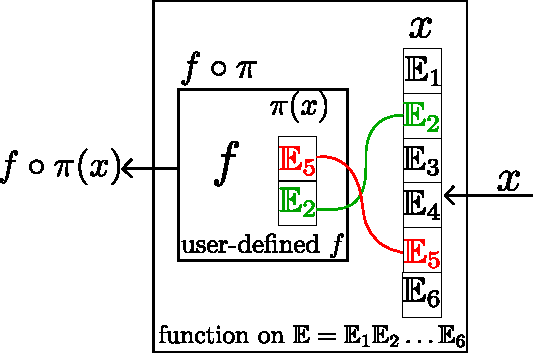
\includegraphics[width=.5\linewidth]{Chapter4-NewPG/Figs/auto_mapping_text.pdf}
\caption{automatic variable mapping}
\label{fig:auto_map}
\end{figure}

\section{Problem Generator}
\label{problem_generator}

The problem generator is the tool constructing the optimization problem.
It registers all the variables and the functions related to a given problem.
Each function is likely to bring additional variables with it.
For each contact contributing to the balance, a variable on $\mathbb{R}^3$ representing the contact force is added to the problem.
The associated wrench is added to the stability constraints.
Once the registration is complete, the complete manifold of the problem is generated and uses the information of the Automatic mapping to `plug' each function with the correct sub-manifold.
Subsequently, the optimization problem can be generated and passed to the solver.
The communication between the solver and the generated problem is made through the RobOptim framework\footnote{\url{http://www.roboptim.net/}}~\cite{moulard:jsme:2013, moulard:jrsj:2014}.

\section{Problem formulations}
\label{sec:problem_formulations}

Let $q=[q_F^T; q_r^T]\in\mathbb{R}^3\times SO(3)\times \mathcal{M}_r$ be the combination of the free-flyer of the robot $q_F\in \mathbb{R}^3 \times SO(3)$ and the articular parameters $q_r\in\mathcal{M}_r$.
Let $\mathcal{W}_i(p)=\{f_i,m_i(p)\}$ be the wrench (force+moment) applied by the environment onto the robot at contact $i$ and expressed on point $p$.
A frame $F$ is composed of a reference point and an orthonormal basis of 3 vectors $F = \{O, (x, y, z)\}$.

Here is a list of constraints that we consider in our problem (implementation of other ones is on-going):
\begin{itemize}
\item Joint limits ${q^-} \leq q_r \leq {q^+}$:\\
These cannot be directly translated on manifolds other than $\mathbb{R}^n$.
For example, spherical joints can be parametrized on $S2 \times \mathbb{R}$, then the $S2$ part can be limited by a cone, and the $\mathbb{R}$ part can have real bounds.
\item The contact constraint consists in identifying the features of two frames $F_1$ and $F_2$.
For example, for a planar contact, we get the set of equation~\ref{eq:planar_contact}.

\begin{equation}
  \begin{split}
    \overrightarrow{O_1O_2}\cdot\vec{z_1} = 0\\
    \vec{z_2}\cdot\vec{z_1} \leq 0 \\
    \vec{z_2}\cdot\vec{x_1} = 0 \\
    \vec{z_2}\cdot\vec{y_1} = 0
  \end{split}
  \label{eq:planar_contact}
\end{equation}

Note that on $F_2$ only the point $O_2$ and the vector $z_2$ are necessary.
Other types of contacts can be created that way, by equalizing other features, as explained in~\cite{escande:ras:2013}.

\item The stability constraint ensures that the Euler-Newton equation~(\ref{eq:NewtonWrench}) is balanced for the set of external wrenches applied to the robot (gravity $\mathcal{W}_G$ and contact forces $\mathcal{W}_i$).
  \begin{equation}
    \sum_{i}{\mathcal{W}_i(p)} + {\mathcal{W}_G(p)} = 0
    \label{eq:NewtonWrench}
  \end{equation}
  For each contact that bears forces (`stability' contact), a wrench applied on the robot at the contact point is added to the problem.
  That wrench is parametrized on a subset of $\mathbb{R}^6$ depending on the type of contact.
  For punctual contacts, the moment part is null on the application point.
  Only a parametrization of the force part on $\mathbb{R}^3$ is needed.
  We model planar contacts as a combination of punctual forces applied at each vertex of the contact polygon.
  In the case of interaction forces between 2 robots, only one wrench is created and it is used as is in the stability equation of one robot and its opposite is used for the stability of the second robot.

\item The friction cone constraint limits the tangential part of every forces to avoid slippage.
We write it as~\ref{eq:friction} (with $\mu$ the friction coefficient)
\begin{equation}
  \begin{split}
    \mu^2f_z^2-f_x^2-f_y^2 \geq 0 \\
    f_z \geq 0
  \end{split}
  \label{eq:friction}
\end{equation}
\end{itemize}

The frame in which the constraints are written matters critically.
Most often, the frame's configuration depends on a part of the optimization variables, that must be accounted for in computing the constraints' Jacobian.
Our framework computes such dependencies automatically.

Our current PG (i.e.\ coding state) does not include yet collisions and auto-collisions, nor torque limits.
Their implementation is on-going and is simply the matter of coding time.
Another important part is its cost function.
We only mention the cost function that have specificities when dealing with manifolds, the distance to a reference posture $q_0$.
On a robot that has all its articulations parametrized on $\mathbb{R}$ the distance can be expressed simply with the Euclidean norm $d = \norm{q_j-q_0}^2$.
Since we work on non-Euclidean manifolds, the logarithm function on the manifold must be used.
It gives the distance vector between two points in the tangent space, the norm of this vector can be used as a distance.
So we get $d = \norm{\text{log}_{q_0}(q_r)}^2$.


%FROM HERE IT IS OLD TEXT

%There can be several kinds of contact between a surface of the robot and its environment(which could contain other robots).
%We denote $\mathcal{S}_R$ and $\mathcal{S}_E$ the two surfaces belonging to two bodies $\mathcal{B}_R$, $\mathcal{B}_E$ that are to be put in contact.
%We equip those surfaces with a frame $\mathcal{F} = \{O, (x, y, z)\}$, with $O$ a point of contact on the surface, and $z$ a vector normal to the surface at $O$.
%The transformation that leads from the reference frame of a body $\mathcal{B}$ to the reference frame of a surface $\mathcal{S}$ is denoted $^\mathcal{S}H_\mathcal{B}$.
%Note that those two surfaces do not need to be plane, a curved continous surface would suit as well.
%For a contact to be geometricaly satisfied, the planes defined by $\{O, (x, y)\}$ on both surfaces must be coplanar with normals of opposite directions.
%This can be assured by satisfying the following set of equation:

%\begin{align}
  %\begin{split}
  %(O_R-O_E) . z_E = 0 \\
  %z_R . x_E = 0 \\
  %z_R . y_E = 0 \\
  %z_R . z_E \leq 0
  %\end{split}
  %\label{eq:floating contact}
%\end{align}

%If any(either or both) of the two surfaces in contact is non-plane, finding the exact location of the contact point on the surface is necessary, because then, the normal to the contact is not known in advance.
%In that situation, we propose to paramaterize the contact frame on the surface on a 1 or 2-dimentional manifold.
%\begin{equation}
  %\mathcal{F}(u_S\in \mathcal{M}_S) = \{O(u_S), (x(u_S), y(u_S), z(u_S)\}
%\end{equation}
%Which, depending on the shape, could be $\mathbb{R}^2$ or $S2$.
%In that case, an additional set of variables $u_S\in \mathcal{M}_S$ is added to the optimization problem as well as the constraint set \ref{eq:floating contact} depending on it.

%The floating contact constraint can be extended to fix the contact to a given position and orientation by adding to it the following set of equation that locks the degrees of freedom of rotation around the normal and translation in the tangent plane of the contact:

%\begin{align}
  %\begin{split}
  %(O_R-O_E) . x_E = 0 \\
  %(O_R-O_E) . y_E = 0 \\
  %y_R . x_E = 0 \\
  %x_R . y_E = 0
  %\end{split}
  %\label{eq:fix planar contact}
%\end{align}

%Those two sets of equations \ref{eq:floating contact} and \ref{eq:fix planar contact} can easily be recombined to generate other types of constraints(e.g. fixing only the translation, or only the rotations...).

%For any scenario to be realistic, the robot must satisfy its stability constraint. Given a set of wrenches applied on the robot $\{\mathcal{W}_0, \mathcal{W}_1...,\mathcal{W}_{n_w}\}$.
%The sum of all those wrenches applied on a singular point must be zero.
%For each punctual contact that needs to bear forces, a new wrench is created, that wrench is parametrized by a set of two vectors describing its force $f = (f_x, f_y, f_z)^T \in \mathbb{R}^3$ and moment $m = (m_x, m_y, m_z)^T \in \mathbb{R}^3$ at the contact point.
%We denode $\mathcal{W}_G$ the wrench generated by the weight of the robot: $\mathcal{W}_G(CoM) = \{(0, 0, -mg)^T, (0, 0, 0)^T\}$.
%For any chosen reduction point $p$, the stability constraint writes as follows:

%\begin{equation}
  %\sum_{i=0}^{n_w}{\mathcal{W}_i(p)} + {\mathcal{W}_G(p)} = 0
  %\label{eq:NewtonWrench}
%\end{equation}

%Equation \ref{eq:NewtonWrench} can be rewritten with only vectors as:

%\begin{equation}
  %\begin{split}
  %\sum_{i=0}^{n_w}{f_i} - m g = 0 \\
  %\sum_{i=0}^{n_w}{m_i(p)} + {m_G(p)} = 0
  %\end{split}
  %\label{eq:NewtonForceMoment}
%\end{equation}

%A usual choice of reduction point for those equations is the center of mass of the robot.
%In which case the moment part of the gravity wrench is null.
%In the case of surfacic contact between two plane surfaces, the contact polygon is determined and a punctual force with zero moment is added on each vertex.
%The forces generated on each point need to satisfy the Coulomb friction cone equations which writes as follows for a friction coefficient $c$:

%\begin{equation}
  %\begin{split}
    %c^2 f_z^2 - f_x^2 - f_y^2 \geq 0 \\
    %f_z \geq 0
  %\end{split}
  %\label{eq:FrictionCone}
%\end{equation}

%It is not straightforward to devise a friction limit in terms of moment.
%Which is why, in the current study, we considere that the punctual contacts are perfect and do not generate moment on their application point.
%This translates in fixing the moment variables of the wrench to zero while the force variables still exist.
%In the case of planar contacts, of course, the moment part cannot be ignored.
%But, given a planar polygon in which the contact happens, the wrench generated by this contact can be modeled as a set of punctual forces, one on each vertex of the polygon.
%Which respect the same friction cone equations \ref{eq:FrictionCone} and are taken into account in \ref{eq:NewtonWrench}.

%\section{Posture Generation, variables and architecture}
%\label{sec:posture_generation_variables_and_architecture}

%\section{Problem Formulation}
%\label{sec:problem_formulation}

%\section{Simulation Results}
%\label{sec:simulation_results}

%\section{Parametrization of complex solids on S2}
%\label{sec:parametrization_of_complex_solids_on_s2}

%\section{Potential contacts}
%\label{sec:potential_contacts}

%\section{Optimization of the solvers parameter for a class of problems}
%\label{sec:optimization_of_the_solvers_parameter_for_a_class_of_problems}
